\documentclass{article}


% if you need to pass options to natbib, use, e.g.:
%     \PassOptionsToPackage{numbers, compress}{natbib}
% before loading neurips_2022


% uncomment one of these
% \usepackage{neurips_2022}             % for blind submission
\usepackage{todonotes}
\usepackage{mathtools}
% \usepackage[preprint]{neurips_2022}   % for preprint submission
% \usepackage[final]{neurips_2022}      % for final submission

% to avoid loading the natbib package, add option nonatbib:
\usepackage[nonatbib, preprint]{neurips_2022}
\usepackage[numbers]{natbib}


\usepackage[utf8]{inputenc} % allow utf-8 input
\usepackage[T1]{fontenc}    % use 8-bit T1 fonts
\usepackage{hyperref}       % hyperlinks
\usepackage{url}            % simple URL typesetting
\usepackage{booktabs}       % professional-quality tables
\usepackage{amsfonts}       % blackboard math symbols
\usepackage{nicefrac}       % compact symbols for 1/2, etc.
\usepackage{microtype}      % microtypography
\usepackage{xcolor}         % colors
\usepackage{graphicx}       % for figures
\usepackage{bm}             % for bold math
\usepackage{tikz}           % for diagrams
\usepackage{scrextend}
\usetikzlibrary{positioning}
\usetikzlibrary{arrows.meta}

\graphicspath{ {./img/} }

\title{PonderBayes: Uncertainty-Informed Pondering}


% The \author macro works with any number of authors. There are two commands
% used to separate the names and addresses of multiple authors: \And and \AND.
%
% Using \And between authors leaves it to LaTeX to determine where to break the
% lines. Using \AND forces a line break at that point. So, if LaTeX puts 3 of 4
% authors names on the first line, and the last on the second line, try using
% \AND instead of \And before the third author name.
\author{
  Giulio Starace \\
  13010840 \\
   \And
  Matteo Rosati \\
  13858149\\
   \AND
  Victor Kyriacou \\
  13438700\\
   \And
  Jille van der Togt\\
  12176729\\
}


\begin{document}
% \raggedbottom
\maketitle


\begin{abstract}

By default, neural networks do not adapt their computational power to the complexity of the task at hand. To overcome this \citet{banino_pondernet_2021} proposed PonderNet, a new algorithm that learns to adapt the amount of computation based on the complexity of the problem. However, PonderNet is still limited to pointwise predictions, with no notion of uncertainty which may be valuable for pondering decisions. We explore approaches for a Bayesian treatment of PonderNet to quantify and exploit model uncertainty in pondering decisions. We implement four ensemble-based variants, one of which achieves higher accuracy and faster convergence time on varying difficulty levels of the same task. We also consider a more complete Bayesian treatment of the problem but ultimately run into variance and numerical stability issues. We hope future work can address our shortcomings and improve this area further.
\end{abstract}


\section{Introduction} \label{introduction}

Machine learning system design almost always involves calibrating the complexity of a model with the complexity of a task. This is typically addressed with hyperparameter depth decisions for linear networks and sequence length in Recurrent Neural Networks (RNNs). This is however sensitive to the biases of human researchers and may lead to sub-optimal configurations. PonderNet \citep{banino_pondernet_2021} attempts to endow neural networks with the ability (referred to as “pondering”) to adjust their computational resource use based on the complexity of the task at hand. It improves on the previously introduced concept of Adaptive Computational Time (ACT) \citep{graves_adaptive_2017} by providing a method to backpropagate through all computational steps with unbiased gradients, as well as providing more stability.

While PonderNet provides a promising step in the direction of more general artificial intelligence, its performance in tasks such as identifying conditional dependencies and dealing with uncertainty is still limited in many of the same ways as conventional Deep Learning (DL) models. We hypothesize that uncertainty may provide useful information in the context of pondering. Bayesian Deep Learning (BDL) has recently emerged as a paradigm to address this issue \citep{murphy_machine_2012, blundell_weight_2015, louizos_multiplicative_2017, fortuin_priors_2022} by using Bayes' Theorem \citep{bayes_lii_1763} to infer a posterior distribution over the model parameters given the observed data. Among others, this allows quantifying a model's uncertainty over its weights and ultimately over its outputs.

In this work, we explore avenues for a Bayesian treatment of PonderNet. We reason that a model that ponders should have some notion of its uncertainty to determine how long it should expect to ponder given its current state. With this premise, we deliver the following contributions:
\begin{enumerate}
    \item We reproduce the findings of the original PonderNet paper, providing code for the model (not released by the authors) and the rest of our work\footnote{\label{note1}\href{https://github.com/thesofakillers/ponder-bayes}{https://github.com/thesofakillers/ponder-bayes}}.
    \item We verify PonderNet's robustness by applying it to a new benchmark, MNIST \cite{deng_mnist_2012}.
    \item We propose four ``ensemble'' PonderNet variants for uncertainty quantification and exploitation, described in Section \ref{ensemble}. Our lambdaGT variant outperforms PonderNet.
    \item We explore the feasibility of a more complete Bayesian treatment of the problem through Stochastic Variational Inference (SVI) as described in section \ref{pyro}.
\end{enumerate}

\section{Related work} \label{related-work}

\subsection{Dynamic Neural Networks}
PonderNet and ACT are part of the broader field of Dynamic Neural Networks (DynNNs). DynNNs distinguish themselves from more conventional static Neural Networks (NNs) in that they can adapt their parameters and/or architecture during inference time based on the incoming inputs. This leads to improvements in computational efficiency, as the networks can dynamically allocate model components such as layers \citep{huang_multi-scale_2018}, channels \citep{lin_runtime_2017} or entire subnetworks \citep{shazeer_outrageously_2016}. DynNNs have also demonstrated improvements in data efficiency in the context of few-shot learning \citep{bertinetto_learning_2016-1, wang_tafe-net_2019}. Adaptive Early Exit Networks \citep{bolukbasi_adaptive_2017} modify the forward pass of an existing network. More classical approaches involve Spiking Neural Networks (SNNs) \citep{maass_networks_1997, izhikevich_simple_2003} which perform data-dependent inference by propagating pulse signals. For a more comprehensive overview of the field, readers are directed to the excellent survey by \citet{han_dynamic_2021-1}.

\subsection{Bayesian Deep Learning}
Like DynNNs, the field of BDL has emerged to address the limitations of more conventional NNs. While DL has achieved tremendous advancements in \textit{perception} tasks, Probabilistic Graphical Models (PGM) have instead been excelling in probabilistic or causal \textit{inference} and at dealing with uncertainty. BDL provides a principled probabilistic framework for unifying PGM and DL to reap the benefits from both fields. Examples include Bayesian interpretations of DL techniques such as dropout \citep{gal_dropout_2016} and ensembling \citep{lakshminarayanan_simple_2017}. Initial research mostly focused on addressing the issue of the nontrivial time complexity of BDL methods \citep{mackay_practical_1992, neal_bayesian_2012}. More recent advancements such as expectation propagation \citep{hernandez-lobato_probabilistic_2015} and the reparametrization trick \citep{blundell_weight_2015, kingma_auto-encoding_2014} have addressed scalability issues leading to more widespread practical adoption of BDL methods. For a more complete overview, we direct readers to the surveys by \citet{wang_survey_2020} and \citet{fortuin_priors_2022}.

While the notion of ``dynamic'' Bayesian networks exists in the form of stochastic processes and other works \citep{rimella_dynamic_2020}, here ``dynamic'' refers to temporal or sequential. To our knowledge, we are the first to consider a Bayesian treatment of a ``dynamic'' neural network in terms of computation adaptation.

\section{Experimental Setup}\label{experimental-setup}

To evaluate the capacity to adapt computation to more difficult tasks, \citet{banino_pondernet_2021} distinguish between \textit{interpolation} and \textit{extrapolation} tasks. In the former, the training and evaluation data share the same difficulty. In the latter, the evaluation data is in some way more difficult. We apply this scheme to two datasets, which we describe in Section \ref{datasets}, comparing PonderNet to our contributed models, which we describe in Section \ref{models}.

\subsection{Datasets and Evaluation} \label{datasets}
To test robustness, we apply PonderNet (but none of our variants) to MNIST \citep{deng_mnist_2012}, a dataset that the original authors did not consider. MNIST consists of 28x28 grayscale images of handwritten digits, with 60,000 training and 10,000 testing samples. The task is to classify a given image as one of the digits between 0 and 9. For interpolation, we leave the inputs untouched for both training and testing. For extrapolation, we randomly rotate the testing set images by degrees in the range $[-112, 112]$.

To aid with comparison, we apply all our models to the parity task used by \citet{banino_pondernet_2021}, originally introduced by \citet{graves_adaptive_2017}. Here the data consists of $P$-dimensional vectors of which a random number of elements $Q \geq 1$ is set to $1$ or $-1$, and the remaining elements are set to 0. The task is to output $1$ if there is an odd number of ones (including negatives) and $0$ if there is an even number. In the \textit{interpolation} setting, $Q \in \{1, \dots, P\}$ for both training and evaluation samples. In the \textit{extrapolation} setting, $Q \in \{1, \dots, P/2\}$ during training and $Q \in \{P/2+1, \dots, P\}$ during evaluation. For our work, we set $P=16$ for interpolation and $P=24$ for extrapolation\footnote{\citet{banino_pondernet_2021} use $P=64$ for interpolation and $P=96$ for extrapolation. In our experimentation, we found that using smaller numbers did not make a difference other than reducing training time.}. For both interpolation and extrapolation, we generate 128,000 training samples and two pairs of 25,600 samples, one for validation and one for testing, ensuring that the difficulty (number of non-zero elements) is uniformly distributed in our dataset. In both cases, we evaluate the halting step (explained in Section \ref{pondernet}), prediction accuracy, and training time metrics.


\begin{figure}[ht]
\centering
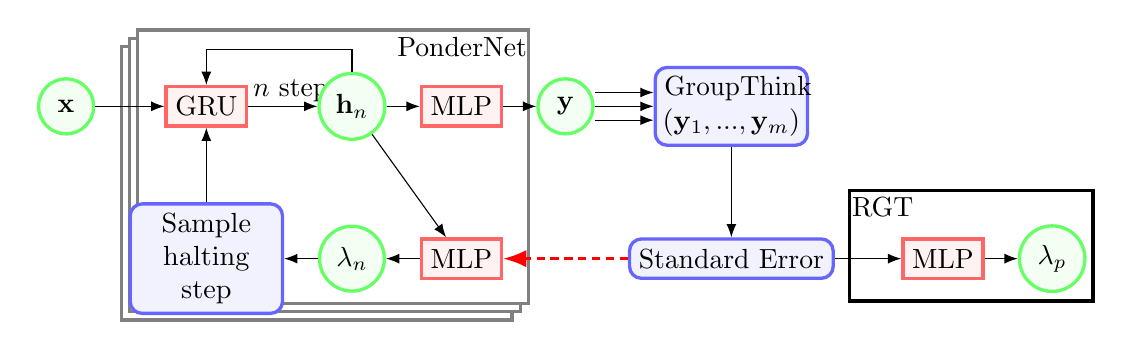
\begin{tikzpicture}[scale = 0.4,
roundnode/.style={circle, draw=green!60, fill=green!5, very thick, minimum size=7mm},
squarednode/.style={rectangle, draw=red!60, fill=red!5, very thick, minimum size=5mm},
operation/.style={rectangle, rounded corners=1ex, draw=blue!60, fill=blue!5, very thick, minimum size=5mm},
]
% \draw[help lines,step=20pt,gray!20] (-20,-4) grid (20,4);
\draw[gray, very thick, fill=white!60] (-398pt,-117pt) rectangle (-45pt,130pt);
\begin{scope}[transform canvas={yshift=+3pt, xshift = +3pt}]
  \draw[gray, very thick, fill=white!60] (-398pt,-117pt) rectangle (-45pt,130pt);
\end{scope}
\begin{scope}[transform canvas={yshift=+6pt, xshift = +6pt}]
  \draw[gray, very thick, fill=white!60] (-398pt,-117pt) rectangle (-45pt,130pt);
\end{scope}
\draw[black, very thick] (260pt,-100pt) rectangle (480pt,0pt);
%Nodes
\node at (-90pt, 130pt) {PonderNet};
\node at (-240pt, 90pt) {$n$ steps};
\node at (290pt, -15pt) {RGT};
\matrix[column sep=12pt, row sep=20pt] (m) {
\node[roundnode]        (x)    {$\mathbf{x}$}; & 
\node[squarednode]      (gru)            {GRU}; &  
\node[roundnode]        (h)              {$\mathbf{h}_n$};& 
\node[squarednode]      (output)   {MLP}; &
\node[roundnode]        (y)     {$\mathbf{y}$}; & 
\node[operation]      (groupthink)   [text width=1.7cm, align=center]{GroupThink ($\mathbf{y}_1, ..., \mathbf{y}_m$)}; &  &  \\
  & \node[operation]      (halt)  [text width=1.7cm, align=center] {Sample halting step}; &
\node[roundnode]        (lambda_n)      {$\lambda_n$}; &
\node[squarednode]      (lambda_layer)   {MLP}; & 
   & \node[operation]      (stderr)   {Standard Error}; & 
& \node[squarednode]      (prior)   {MLP}; & \node[roundnode]        (lambda_p)     {$\lambda_p$}; \\
};
%Lines
\draw[-Latex] (x.east) -- (gru.west);
\draw[-Latex] (gru.east) -- (h.west);
\draw[-Latex] (halt.north) -- (gru.south);
\draw [-Latex](h.north) -- ++(0, 20pt) -| (gru.north);
\draw[-Latex] (h) edge (lambda_layer);
\draw[-Latex] (lambda_layer.west) -- (lambda_n.east);
\draw[-Latex] (lambda_n.west) -- (halt.east);
\draw[-Latex] (h.east) -- (output.west);
\draw[-Latex] (output.east) -- (y.west);
\draw[-Latex] (y.east) -- (groupthink.west);
\begin{scope}[transform canvas={yshift=.5em}]
  \draw[-Latex] (y.east) -- (groupthink.west);
\end{scope}
\begin{scope}[transform canvas={yshift=-.5em}]
  \draw[-Latex] (y.east) -- (groupthink.west);
\end{scope}
\draw[-Latex] (groupthink.south) -- (stderr.north);
\draw[-Latex] (stderr.east) -- (prior.west);
\draw[-Latex] (prior.east) -- (lambda_p.west);
\draw[very thick, densely dashed, red, arrows = {-Latex}] (stderr.west) -- (lambda_layer.east);
\end{tikzpicture}
\caption{A graphical representation of the implemented models on the parity task modifying the original PonderNet model. The red dashed arrow represents the lambdaGT model, i.e., the standard error from GroupThink being used for the input to the $\lambda_n$ layer. The additional architecture implemented in RGT and aRGT can be found in the black rectangle.}
\label{fig:models}
\end{figure}

\subsection{Models} \label{models}

The following section describes PonderNet, which our work is based on, and our extensions.

\subsubsection{PonderNet} \label{pondernet}
PonderNet \citep{banino_pondernet_2021} considers a supervised setting where the goal is to learn a function $f : x \rightarrow y$ from data $(\textbf{x},\textbf{y})$ with $\textbf{x} = \{x^{(1)}, \ldots, x^{(k)}\}$ and $\textbf{y} = \{y^{(1)}, \ldots, y^{(k)}\}$. The authors propose a new architecture that adjusts the forward pass and is trained using a custom loss function. The architecture requires a \textit{step function} $s$ of the form $\hat y_n, h_{n+1}, \lambda_n = s(x,h_n)$ and an initial state $h_0$, where $\hat y_n$ and $\lambda_n$ are the network outputs and scalar probability of ``halting'' at step $n$. 

PonderNet uses $\lambda_n$ to learn the optimal value for $n$ and uses a Bernoulli random variable $\Lambda_n$ in order to represent a ``continue'' ($\Lambda_n$ = 0) state and a terminal ``halt'' ($\Lambda_n$ = 1) state. The decision process starts at a ``continue'' state with the transition probability  
\begin{equation}
    P(\Lambda_n=1 | \Lambda_{n-1}=0) = \lambda_n \quad \forall~1 \leq n \leq N.
\end{equation}
In words, this is the conditional probability of entering a ``halt'' state at step $n$ given that there has been no previous halting.

The prediction $\hat y \sim \hat Y$ is sampled with $P(\hat Y = \hat y_n) = p_n$, where 
\begin{equation}
    p_n = \lambda_n \prod_{j=1}^{n-1}(1-\lambda_j).
\end{equation}
Here $p_n$ is a geometric probability distribution estimating the probability that halting has occurred at steps $0, \dots, N$, where $N$ is a hyperparameter setting the maximum number of ponder steps available to the model. In Fig. \ref{fig:models}, PonderNet is illustrated in the grey box.

To train PonderNet, the sum of a reconstruction loss $L_{\textsc{Rec}}$ and regularization loss $L_{\textsc{Reg}}$ is optimized:

\begin{equation}\label{eq:ponderloss}
    L = \underbrace{\sum_{n=1}^N p_n \mathcal{L}(y, \hat y_n)}_\text{$L_{\textsc{Rec}}$} + \beta \underbrace{ \text{KL}(p_n || p_G(\lambda_p))}_\text{$L_{\textsc{Reg}}$},
\end{equation}


$L_{\textsc{Rec}}$ is equivalent to the expected reconstruction loss across the ponder steps, where $\mathcal{L}$ can be any arbitrary loss function.  $p_G(\lambda_p)$ is a pre-determined prior geometric distribution parameterized by the hyperparameter $\lambda_p$. By using the $\text{KL}$ divergence \cite{kullback_information_1951} between $p_n$ and $p_G$, $L_{\textsc{Reg}}$ not only biases the network toward the expected number of ponder steps $1/\lambda_p$ but also promotes exploration by incentivizing non-zero probability of halting for each step. $\beta$ is an additional hyperparameter, scaling the regularization loss contribution. 

\paragraph{Training Details} For the parity task, we use a gated recurrent unit (GRU) cell \citep{chung_empirical_2014} with 128 hidden units. We set $\lambda_p = 0.2$ and $\beta=0.01$ and minimize binary cross-entropy for $\mathcal{L}$ using the Adam optimizer \citep{kingma_adam_2017-1} with learning rate 0.0003 and clip gradient norms at 1 for numerical stability. We train for 80,000 steps using a batch size of 128 and use the model with the highest validation halted step accuracy for evaluation. For MNIST, we make use of the same setup but first pass our inputs through a Convolutional Neural Network (CNN)\footnote{We use two convolutional layers mapping from 10 to 20 channels using a kernel size of 5, with a dropout layer \citep{srivastava_dropout_2014} with $p=0.5$ in between. We pass our outputs to a dense layer that maps to 64 dimensions. We use ReLU as our activation function throughout.} to generate 64-dimensional embeddings as input to our GRU cell. Here we use cross-entropy instead of binary cross-entropy and train for 20,000 steps.

\subsubsection{Ensemble Models}\label{ensemble}
Inspired by \citet{lakshminarayanan_simple_2017}, we consider ``ensembles'' for uncertainty quantification. An ensemble model employs a group (or ``ensemble'') of $E$ deterministic NNs and uses some combination of the models' predictions as its output. The different point estimates can be considered different modes of the Bayesian posterior \citep{jospin_hands-bayesian_2022}. One can recover from these point estimates the standard deviation $\sigma$ and hence standard error $\text{SE} = \sigma / \sqrt{E}$, thus quantifying uncertainty. We developed four different architectures in this fashion, which are outlined below. We set $E = 5$ in all our models. We illustrate ensembling in \ref{fig:models} via the layering of the PonderNet boxes.

\paragraph{GroupThink} \textit{GroupThink} consists of $E$ PonderNet modules, each trained independently using its own instance of the optimizer and loss mentioned in Section \ref{pondernet}. When receiving an input, GroupThink passes it to each module, generating an output from each of them. The mean prediction is taken, and a standard error can be quantified as described above.

\paragraph{Rational GroupThink (RGT)} GroupThink does nothing with the uncertainty it quantifies. The intuition behind RGT is that a more uncertain PonderNet should expect to ponder for longer and vice-versa. RGT attempts to do this by using its uncertainty to update its prior. More specifically, RGT treats the standard error computed at training step $t$ as input data to a separate sigmoid-activated linear layer trained to compute the appropriate $\lambda_p$ value for the (now dynamic) regularization loss in training step $t+1$. Because $\lambda_p$ is now learned and shared across the $E$ models, the computational graph must be retained when training the first $E-1$ models. Apart from eliminating a hyperparameter, we hypothesize that allowing the model to update its priors should lead to increased performance due to the increased flexibility that is afforded.

\subparagraph{Annealed RGT (aRGT)} RGT shares the same loss configuration as PonderNet and thus only weakly weighs the regularization term ($\beta=0.01$). This is, however, the only term that contributes to the optimization of $\lambda_p$ and should be weighted more strongly if a greater exploration of $\lambda_p$ values is desired. We conjecture that our $L_{\textsc{Reg}}$ term should be more strongly weighted at the beginning of training to encourage the model to explore a more extensive range of $\lambda_p$ but should ultimately return to being dominated by the reconstruction loss. To achieve this, we anneal $\beta$ with the schedule:

\begin{equation}
    A_\beta(e) = \frac{1}{2e + 1 + \gamma} + \gamma
\end{equation}

Where $A_\beta(e)$ is the annealed value of $\beta$ at epoch $e$, an exponentially decreasing value asymptotically approaching the value of $\gamma$, which we set to 0.01 to mimic the effect of $\beta$ in the previous models at later stages of training.

\paragraph{Lambda GroupThink (lambdaGT)} LambdaGT attempts to directly incorporate the uncertainty obtained with ensemble methods in the decision of the models to halt or keep pondering. As shown in Figure \ref{fig:models}, we modify the MLP that outputs $\lambda_n$, the parameter that defines the halting probability distribution, by expanding it to accept as input a concatenated vector of $h_n$ and $\text{SE}_n$. This latter term is the standard error of the ensemble's predicted output at pondering step $n$ for the prior batch. $\text{SE}_n$ for the first batch is initialized as the maximum possible standard error.\footnote{Note that using the prior batch's error may lead to issues of significant variance when training. LambdaGT can be adapted to resolve this by using the same batch in a two-step training process: first, freeze the weights that make use of $\text{SE}_n$ and backpropagate through the rest of the model, calculate $\text{SE}_n$, and second, freeze all other weights and backpropagate through the weights that use $\text{SE}_n$. We find, however, that the naive implementation trains successfully and requires less compute.} The modules can now utilize the uncertainty information between their predictions to improve their halting decisions. As in PonderNet, we regularise the halting probability $p_n$ to follow a geometric distribution $p_G(\lambda_p)$.


\subsubsection{A Fully Bayesian Approach}\label{pyro}

A full Bayesian treatment of PonderNet would enable more complete characterization of uncertainty in the model's predictions. This could be incorporated to decide how much to ponder, similarly as above. We took steps in the direction of such an implementation by leveraging the Pyro probabilistic programming language \citep{bingham_pyro_2019} to transform the output layer of the model into a Bayesian layer. Our goal was, given the dataset $D$ and an input datapoint $x^*$, to learn the posterior predictive distribution
\begin{equation}
    p(y^* | x^*, D) = \int_{W} p(y^* | x^*, W)\, p(W | D)\: dW
\end{equation}
by learning the posterior $p(W | D)$ on the weights $W$ of the layer. We use SVI to estimate this posterior distribution with a multivariate normal $q_{\theta}(W)$ parametrized by $\theta$. We seek to minimize, therefore, the KL divergence between $p(W | D)$ and $q_{\theta}(W)$ which is equivalent to maximizing the evidence lower bound (ELBO) \citep{wingate_automated_2013}. Our $L_{\textsc{Rec}}$ term is replaced by the ELBO and the objective function from (\ref{eq:ponderloss}) becomes:
\begin{equation}
        L = - \sum_{n=1}^N \Big[p_n\,\text{ELBO}(p(W , D), q_{\theta}(W))\Big] + \beta\,\text{KL}(p_n || p_G(\lambda_p)),
\end{equation}
where we conserve the weighted average by the halting probability $p_n$ per step $n$ to adequately add up the contributions of each step and the regularization term to encourage exploration. 

Ultimately, this approach was unsuccessful due to significant variance and a lack of maturity in the development ecosystem. The Bayesian treatment further increased the numerical instability of PonderNet, with its gradients exhibiting extremely high variance and dependence on prior distributions and hyperparameters. Despite our best efforts searching for adequate hyperparameters, this led to little to no learning or numerical instability in the worst cases. Additionally, we found it challenging to navigate the probabilistic programming ecosystem for implementing BDL solutions at a more advanced and customized level.


\section{Results and Analysis} \label{results-and-anal}

\begin{table}[t]
\caption{Average test set accuracy and halting step of the models on the parity datasets for interpolation and extrapolation. The standard error in the metrics from runs using 5 different seeds is also reported.}
\label{tab:test-results}
\centering
\begin{tabular}{rcccc}
\toprule
 & \multicolumn{2}{c}{Test Accuracy} & \multicolumn{2}{c}{Halting Step} \\
 \cmidrule(rl){2-3} \cmidrule(rl){4-5}
 & Interpolation & Extrapolation & Interpolation & Extrapolation \\ \midrule
PonderNet & $0.992 \pm 0.005$ & $0.908 \pm 0.076$ & $8.5 \pm 1.4$ & $10.2 \pm 1.8$ \\
GroupThink & $0.986 \pm 0.009$ & $0.883 \pm 0.049$ & $8.9 \pm 0.3$ & $9.3 \pm 0.3$ \\
RGT & $0.689 \pm 0.084$ & $0.502 \pm 0.001$ & $9.1 \pm 3.1$ & $2.4 \pm 0.2$ \\
aRGT & $0.745 \pm 0.093$ & $0.502 \pm 0.001$ & $6.4 \pm 1.7$ & $3.8 \pm 1.2$ \\
\textbf{lambdaGT} & $\bm{0.995 \pm 0.0002}$ & $\bm{0.919 \pm 0.022}$ & $8.7 \pm 0.3$ & $9.9 \pm 0.3$ \\
\bottomrule
\end{tabular}
\end{table}

\begin{figure}[ht]
\centering
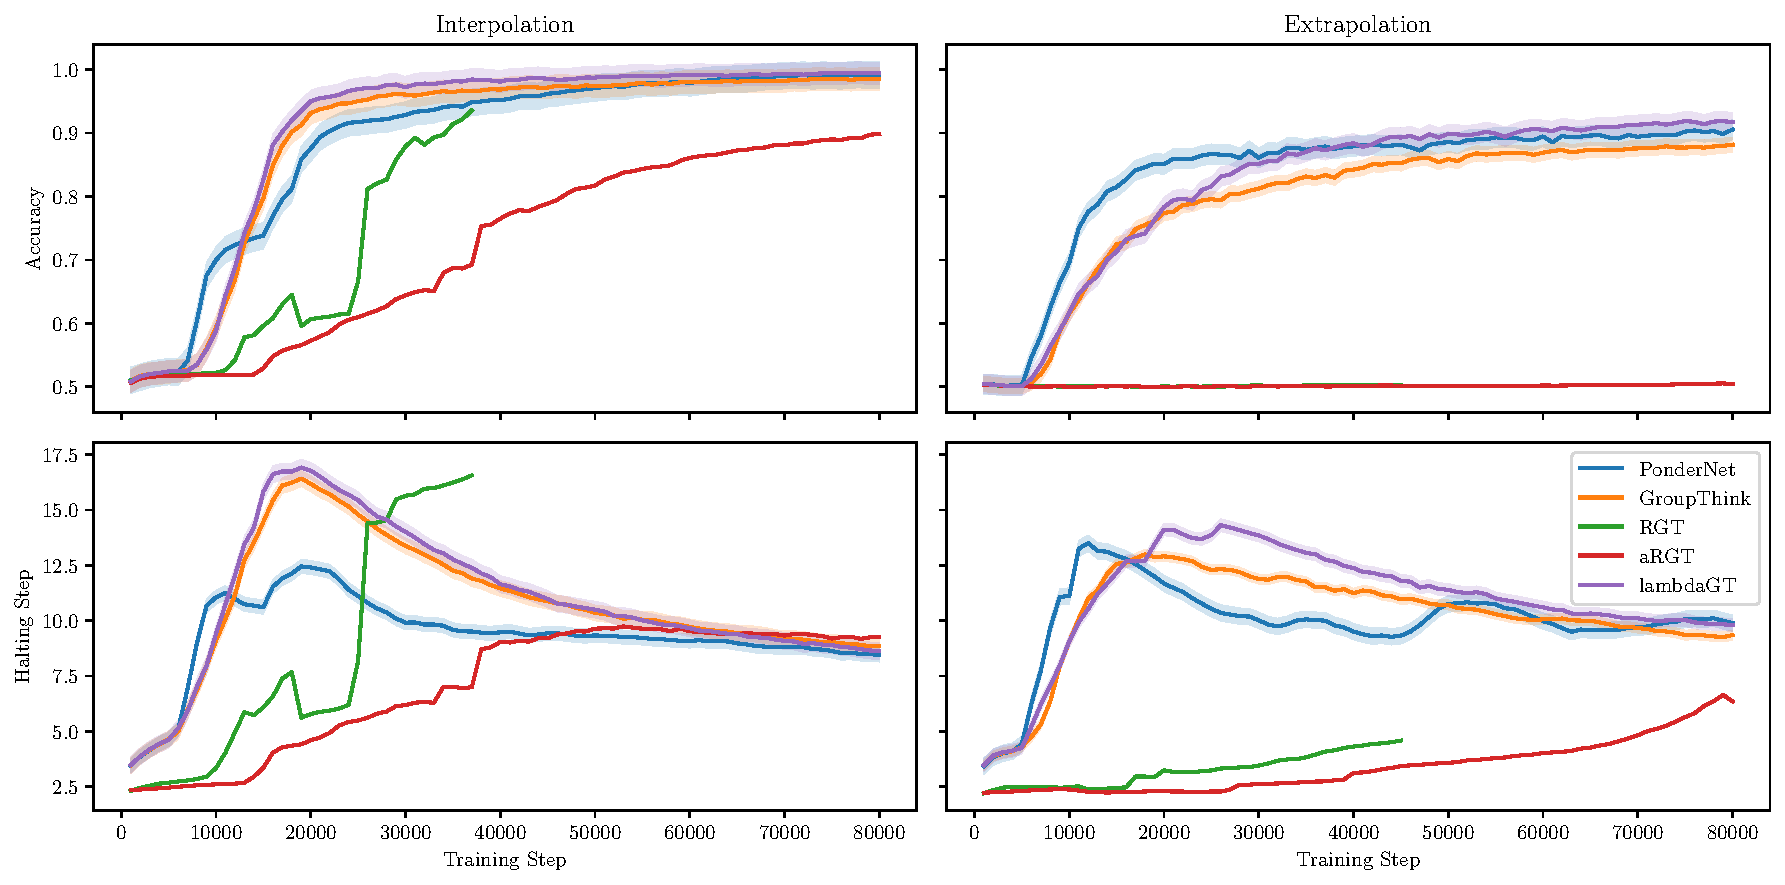
\includegraphics[width=\textwidth]{val_results.pdf}
\caption{Average validation accuracy and halting step during training for the four models, with standard error. Metrics were computed over 5 random seeds. RGT and aRGT suffer from numerical instability causing premature termination and therefore difficulty in seed aggregation.}
\label{fig:timeseries}
\end{figure}

Table \ref{tab:test-results} presents the test accuracy and average halting step of each model presented in Section \ref{models}. We successfully reproduce the results shown in the original paper, with a higher accuracy achieved in interpolation (99.2 \%) than extrapolation (90.8 \%) and a demonstrated adaptation to the more difficult task via the increase in average halting step (10.2 steps vs. 8.5). We verify PonderNet's robustness by observing the same trends on the MNIST dataset. We achieve test accuracies and average halting steps of $99.2\pm0.002~\%$ and $9.1\pm0.1$ in interpolation and $63 \pm 0.004~\%$ and $10.6\pm0.3$ in extrapolation. The much lower extrapolation test accuracy indicates that our image rotation was too challenging compared to the additional non-zero elements in the parity task.

PonderNet matches or outperforms three out of our four ensemble variants. RGT and aRGT suffered in particular to numerical instability, causing several if not all the seeds to halt training prematurely. This can also be noted in Fig. \ref{fig:timeseries}. The annealing proposed in aRGT seems to help, but overall this family of variants misses the mark.

Our lambdaGT variant generally outperforms the rest of the model zoo, marginally improving on the performance of PonderNet. We also note from Fig. \ref{fig:timeseries} that lambdaGT converges earlier than PonderNet on interpolation. This supports our hypothesis that additional information from the model's uncertainty aids learning. LambdaGT accuracies also have the smallest SEs, indicating greater stability across runs. Finally, both lambdaGT and GroupThink explore more halting steps than PonderNet during training, suggesting that the ensemble treatment aids exploration and thus more robust halting step convergence.

We hope future work can successfully apply a complete Bayesian treatment to the problem (as discussed in Section \ref{pyro}) to complete the comparison, perhaps on a new, less saturated task. We also wish to investigate whether lambdaGT outperforms RGT for inherent reasons or whether addressing the numerical instability of the latter could lead to different results. The impact of different initializations of the $\lambda_p$ term or of additional loss terms and training regimens could be avenues to explore to redeem the RGT family.

\section{Conclusion} \label{conclusion}
In this work, we explored approaches for the Bayesian treatment of PonderNet. We replicate the results of the original paper on the parity task and test on MNIST to verify robustness. We then propose, implement and evaluate four ensemble-based methods for uncertainty quantification and exploitation and compare their performance to PonderNet. One of our variants, lambdaGT, outperforms all other models. Future work may leverage a complete Bayesian treatment of PonderNet or investigate more efficient ensembling techniques \cite{garipov_loss_2018}.

\newpage
\bibliography{references.bib} 
\bibliographystyle{abbrvnat}
\newpage
\appendix
\section{Numerical Instability}

A number of the models explored in this work suffer from numerical instability. This is where floating-point errors propagate through our algorithms and cause the resulting malformed input to lead to premature termination. We briefly investigated the source of this numerical instability, as it also seemed to affect PonderNet, as mentioned in \citet{banino_pondernet_2021}'s work. 

For PonderNet and our ensemble models described in Section \ref{ensemble}, we unsurprisingly found the culprit to be vanishing and exploding gradients. Numerical instability was less prevalent in the fully Bayesian approach of Section \ref{pyro}, making it more challenging to reproduce the numerical stability issues consistently. We do however suspect that the source of the issue is ultimately the same, namely the vanishing/exploding gradients issue mentioned earlier.

Aside from the already present gradient clipping, we briefly considered a number of techniques for addressing the issue further. We experimented with using other optimization settings, including 
\begin{itemize}
    \item using vanilla Stochastic Gradient Descent (SGD) with a scheduled learning rate.
    \item using the AdamW optimizer \citep{loshchilov_decoupled_2018}.
    \item Varying the hyperparameters of our Adam-based optimizer, such as the base learning rate or the epsilon term.
\end{itemize}
We also considered employing Batch Normalization \citep{ioffe_batch_2015} and using ReLU whenever sensible. We found that increasing the epsilon term in Adam optimization from $1\mathrm{e}{-8}$ to $1\mathrm{e}{-6}$ generally helped. However, ultimately none of our hotfixes fully solved our issue, often trading stability for learning capabilities. 

Due to a limited budget, we were unable to explore solutions to these issues beyond these hotfixes, but we believe a solution is certainly possible. We hope future work can be dedicated to this direction.

\end{document}
